\documentclass[a4paper,12pt]{report}

%% Color
\usepackage{color}

%% Diagrams
\usepackage{graphicx,epsfig}

%% To control the table caption positioning
\usepackage{caption} 
\captionsetup[table]{skip=5pt}

%% 'H' for exact placement of floats
\usepackage{float}

%% For a lot of maths support, including align
\usepackage{amsmath}

%% For euros
\usepackage{eurosym}

%% Personalisation
\setlength{\parskip}{1em}

\begin{document}

\author{Devrim Gunyel\\
  Department of Computer Science\\
  Maynooth University\\
  Maynooth\\
  Co. Kildare\\
  IRELAND}
\date{\today}
\title{Demo Report}
\maketitle

\begin{abstract}
This is a demo report-style document to show what that looks like. Suitable for a dissertation.
\end{abstract}

\tableofcontents

\newpage

\chapter{Introduction}
\label{intro}

You can include files-e.g. place chapters in separate files, etc.

\section{Lists}

You can find excellent Latex help in the following documents\footnote{Search for them on the web}:
\begin{enumerate}
\item The Not So Short Introduction to \LaTeX $\epsilon$ 
\item \LaTeX Tutorials A Primer
\item \LaTeX2$\epsilon$ for authors
\item Essential \LaTeX++
\item Short Math Guide for \LaTeX
\end{enumerate}

Like html, latex supports both numbered (enumerated) and unnumbered (itemized) lists - you can customise these.
\begin{itemize}
\item normal,
\item {\tiny tiny},
\item {\large large},
\item {\Huge Huge}
\item and {\large various other}
\end{itemize}
font sizes.

\section{Alignment}

\begin{flushleft}
This text is\\ left-aligned.
\LaTeX{} is not trying to make
each line the same length.
\end{flushleft}

\begin{flushright}
This text is right-\\aligned.
\LaTeX{} is not trying to make
each line the same length.
\end{flushright}

\begin{center}
This line is\\at the centre\\of the earth
\end{center}

\section{Font Styles and Colours}

You can use \textbf{bold}, \textit{italics}, \underline{underlining}, super$^{scripts}$ and sub$_{scripts}$.

You can colour the font: {\color{red}{red}, \color{green}{green}, \color{blue}{blue}}, etc. Note this requires a package or ``stylefile'' called color. These packages provides extensions to \LaTeX - there is a large collection of them - you can even write your own.

\section{Figures}

Figures and Tables are called ``floats'' - \LaTeX places them according to various rules. You can provide hints: (h)ere, (t)op, (b)ottom, and by the float package: (H)ere.

Here is a simple figure (see Fig. \ref{fig-demo}).

\begin{figure}[t]
\centerline{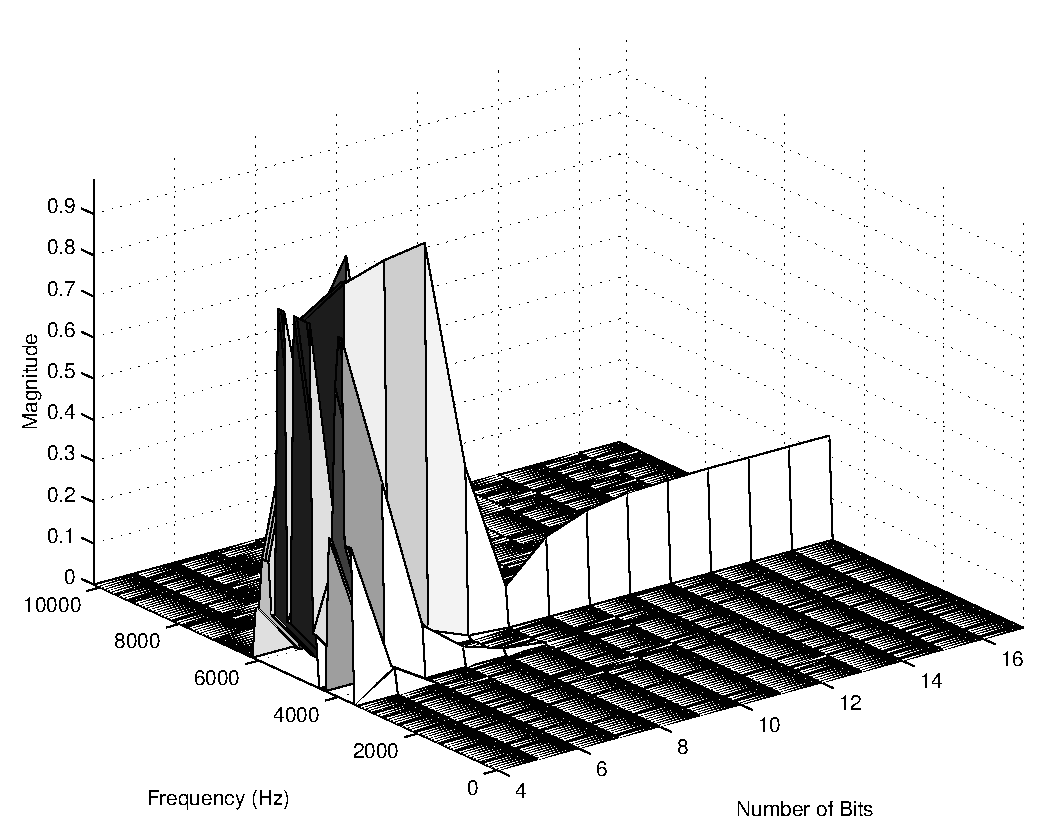
\includegraphics[width=.5\textwidth]{fig1.eps}}
\caption{Demo Figure}
\label{fig-demo}
\end{figure}

You can scale and rotate figures (see Figs. \ref{fig-demon} \ref{fig-demow}).

\begin{figure}[t]
\centerline{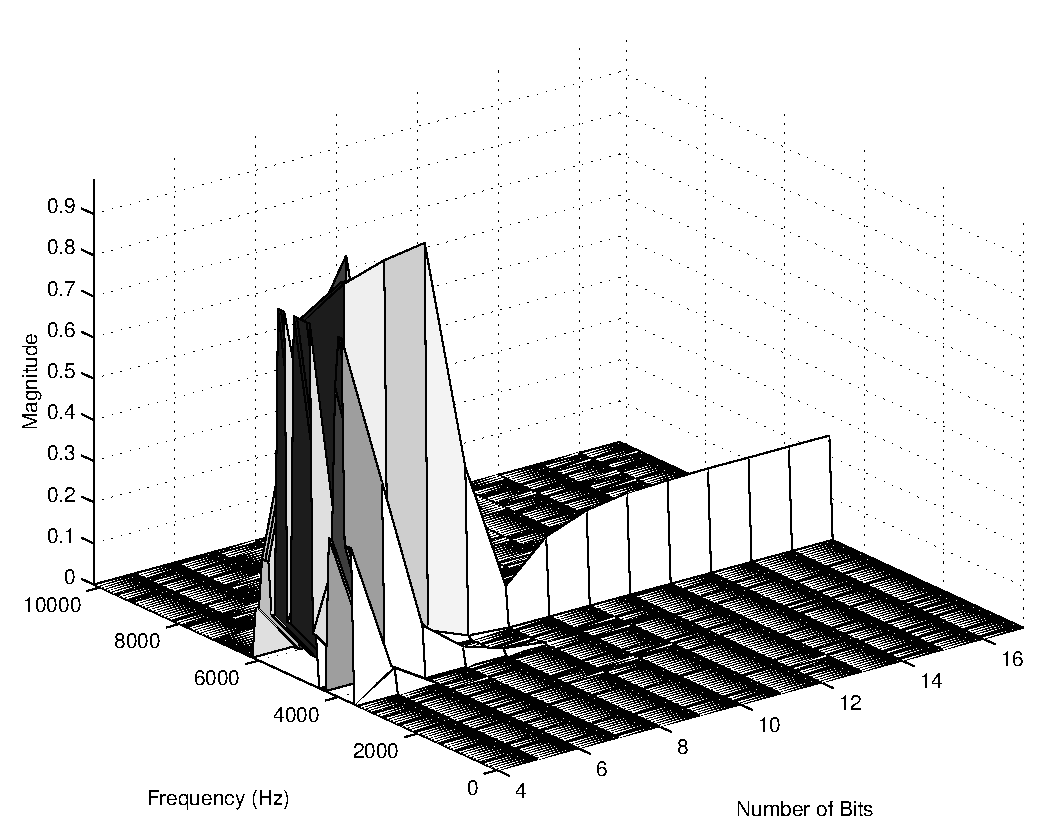
\includegraphics[width=0.1\textwidth]{fig1.eps}}
\caption{Demo Figure-Narrow}
\label{fig-demon}
\end{figure}

\begin{figure}[t]
\centerline{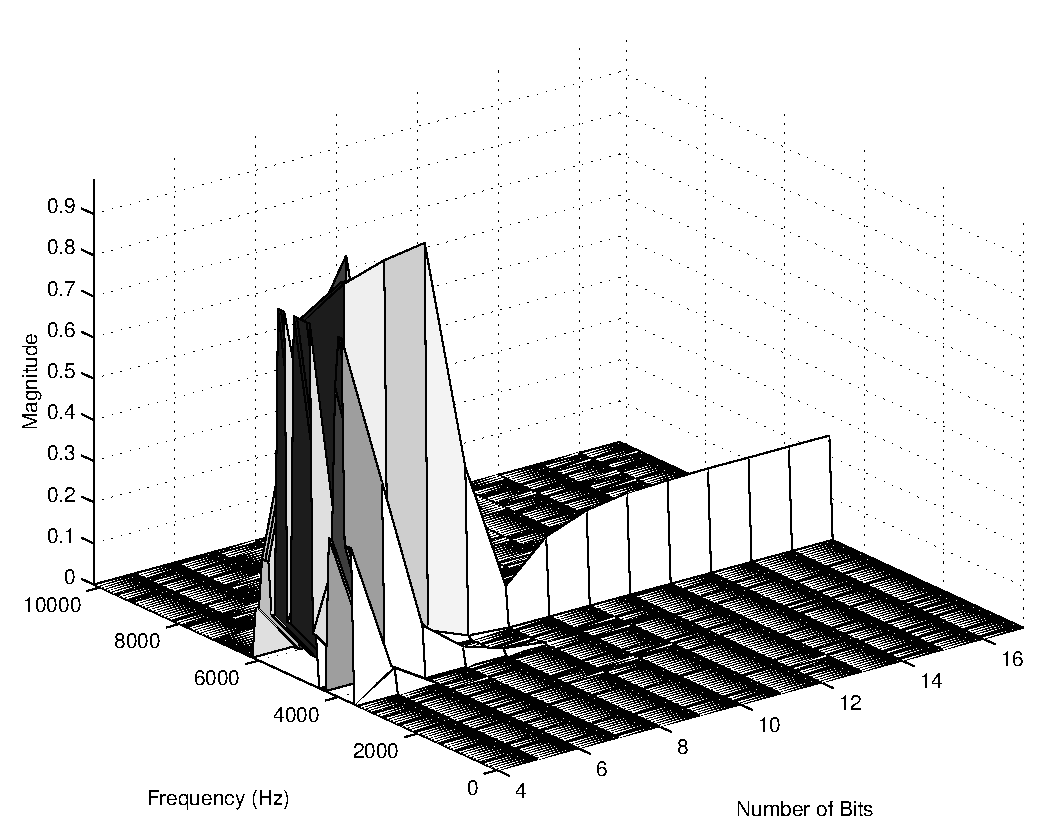
\includegraphics[width=\textwidth]{fig1.eps}}
\caption{Demo Figure-Wide}
\label{fig-demow}
\end{figure}

\begin{figure}[t]
\centerline{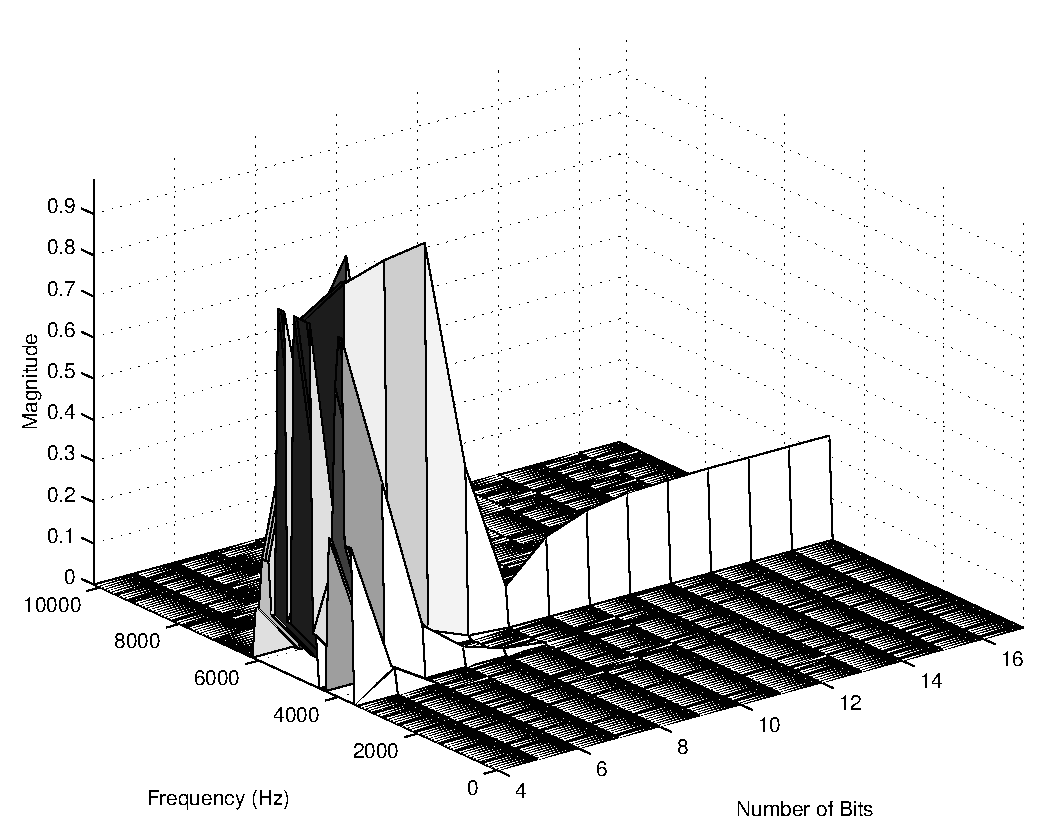
\includegraphics[width=.5\textwidth,angle=45]{fig1.eps}}
\caption{Demo Figure-Rotated}
\label{fig-demo45}
\end{figure}

And add borders (see Fig. \ref{fig-demob}).

\begin{figure}[!htbp]
\centerline{
\fbox{
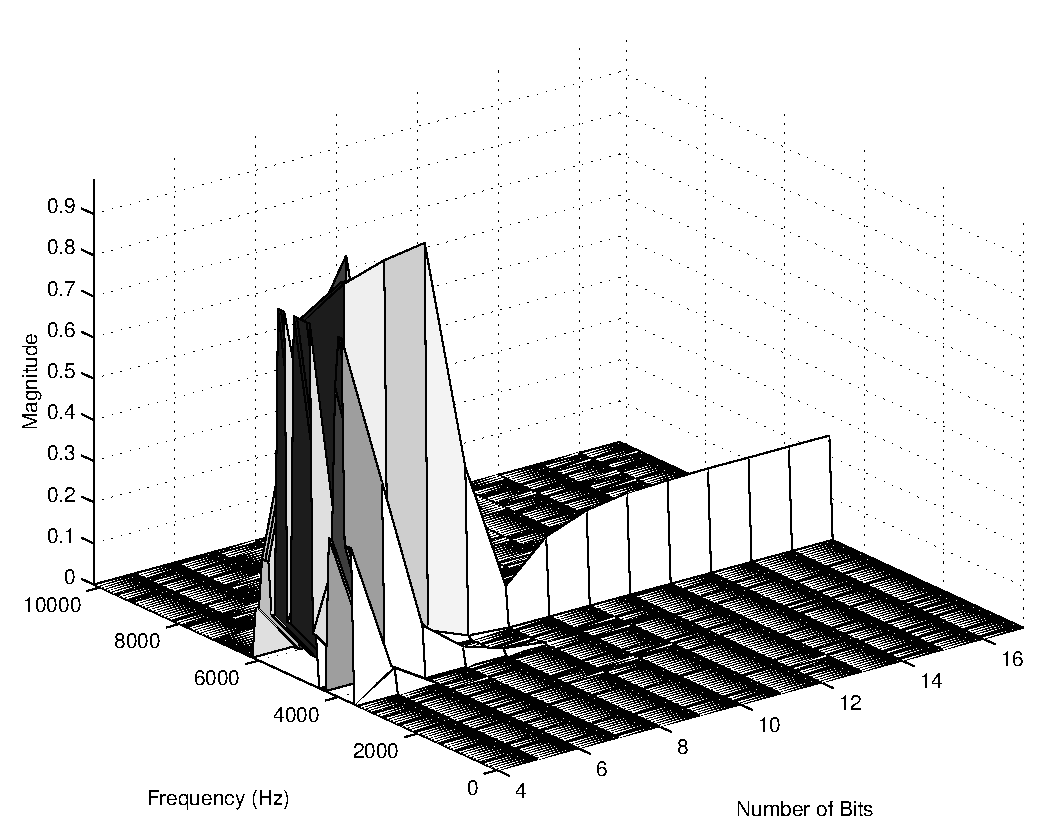
\includegraphics[width=0.5\textwidth]{fig1.eps}}
}
\caption{Demo Figure-With Border}
\label{fig-demob}
\end{figure}

Note: !htbp means:
\begin{description}
\item[!] place as early as possible
\item[h] place here if can
\item[t] otherwise at top of page
\item[b] otherwise at bottom of page
\item[p] otherwise on a float page.
\end{description}

\subsection{Useful Tools}

Useful figure tools: gnuplot\footnote{Can create \LaTeX pictures}, xfig, gimp, \textbf{inkscape}, powerpoint, excel.

\subsection{Floats}

Note that figures are \textit{floats} - Latex decides exactly where to place them: the \textbf{h}, \textbf{t} and \textbf{b} are hints, but \textbf{H} means Here, even if a page-break is required. If enough figures get queued up, they are all presented at the end of the chapter (or use the \textbackslash clearpage command).

\clearpage

\section{Tables}

See Table \ref{table-demo} for an ``example'' table. Note the smart-quotes. Note that tables are also \textit{floats} and are placed automatically, unless you use ``H''.

\begin{table}[H]
\centering
\caption{This is a Table}
\begin{tabular}{|l|c|r|}
\hline
\textbf{ID} & \textbf{Data} & \textbf{Value} \\
\hline
Line 1 & data for line 1 & 189\\
\hline
Line 1 & data for line 1 & 88\\
\hline
\end{tabular}
\label{table-demo}
\end{table}

You can do all sorts of complex things with tables: multi-row, multi-column, multi-page (with the header rows repeated), etc.

\chapter{Background}

You can reference any label in the document - for example, the tables are shown in Ch. \ref{intro}.

You can cite works in the reference section \cite{Medina:2009} and \cite{Wilkes:1951}.

Note: the bibliography would normally be in a separate 'bibtex' file, except for very small documents. There are various databases and utilities to help with references also-especially useful when a group is building up a shared list.

\chapter{My Work}

\section{Maths Mode and Symbols}

\LaTeX is excellent at typesetting maths, equations etc. You can reference equations - see Eqn. \ref{eq-pyth}.

\begin{equation}
\label{eq-pyth}
x^2 = y^2 = z^2
\end{equation}

Or place maths inline: $E=mc^2$, with no equation numbering.

\begin{itemize}

\item You can use \underline{greek} and \textit{other} letters: $\alpha \beta \delta$ \euro \copyright

\item There is a large set of maths symbols: $\Rightarrow \bigodot \iff \mapsto \overrightarrow{AB} \pm \Pi$, etc.

\item Set operators: \[A \subset B\].

\item Sums: \[x = \sum_{i=0}^{\inf}\left(\frac{1}{i}\right)\]

\item Integrals: \[x = \int_{i=0}^{\infty}\big(\frac{1}{i}\big)\]

\item arrays, matrices, etc: 

\[
\begin{bmatrix}
1 & 2 & 3 \\
4 & 5 & 6 \\
7 & 8 & 9
\end{bmatrix}
\]

\begin{equation*}
|x| = \left\{
\begin{array}{rl}
-x & \text{if } x < 0\\
0 & \text{if } x = 0\\
x & \text{if } x > 0
\end{array} \right.
\end{equation*}

\item And alignment to (for example) the = sign:

\begin{align*}
f(x) &= (a+b)(a-b) \\
&= a^2-ab+ba-b^2 \\
&= a^2+b^2 
\end{align*}

\end{itemize}

\section{Verbatim}

Verbatim allows for untranslated text - see Appendix \ref{app-SC}.

\section{Boxes}

\framebox[10cm][c]{
   Use boxes, and
   \framebox[5cm][c]{
      nested
      \framebox[2cm][c]{boxes}
   }
}

\section{Pictures}

You can also draw lines and other shapes in pictures - these scale really well, as they are vector graphics. Note how figures float, but raw pictures don't.

\begin{center}
\begin{figure}
\label{fig-p1}
\begin{center}
\setlength{\unitlength}{5cm}
\begin{picture}(1,1)
\put(0,0){\line(0,1){1}}
\put(0,0){\line(1,0){1}}
\put(0,0){\line(1,1){1}}
\put(0,0){\line(1,2){.5}}
\put(0,0){\line(1,3){.3333}}
\put(0,0){\line(1,4){.25}}
\put(0,0){\line(1,5){.2}}
\put(0,0){\line(1,6){.1667}}
\put(0,0){\line(2,1){1}}
\put(0,0){\line(2,3){.6667}}
\put(0,0){\line(2,5){.4}}
\put(0,0){\line(3,1){1}}
\put(0,0){\line(3,2){1}}
\put(0,0){\line(3,4){.75}}
\put(0,0){\line(3,5){.6}}
\put(0,0){\line(4,1){1}}
\put(0,0){\line(4,3){1}}
\put(0,0){\line(4,5){.8}}
\end{picture}
\caption{Example Picture}
\end{center}
\end{figure}

\setlength{\unitlength}{1mm}
\begin{picture}(60, 40)
\put(20,30){\circle{1}}
\put(20,30){\circle{2}}
\put(20,30){\circle{4}}
\put(20,30){\circle{8}}
\put(40,30){\circle{1}}
\put(40,30){\circle{2}}
\put(40,30){\circle{3}}
\put(40,30){\circle{4}}
\put(40,30){\circle{5}}
\put(40,30){\circle{6}}
\put(40,30){\circle{7}}
\put(40,30){\circle{8}}
\put(40,30){\circle{9}}
\put(40,30){\circle{10}}
\put(40,30){\circle{11}}
\put(40,30){\circle{12}}
\put(40,30){\circle{13}}
\put(40,30){\circle{14}}
\put(15,10){\circle*{1}}
\put(20,10){\circle*{2}}
\put(25,10){\circle*{3}}
\put(30,10){\circle*{4}}
\put(35,10){\circle*{5}}
\end{picture}

\fbox{
\setlength{\unitlength}{0.75mm}
\begin{picture}(70,50)
\put(30,20){\vector(1,0){30}}
\put(30,20){\vector(4,1){20}}
\put(30,20){\vector(3,1){25}}
\put(30,20){\vector(2,1){30}}
\put(30,20){\vector(1,2){10}}
\thicklines
\put(30,20){\vector(-4,1){30}}
\put(30,20){\vector(-1,4){5}}
\thinlines
\put(30,20){\vector(-1,-1){5}}
\put(30,20){\vector(-1,-4){5}}
\put(0.3,45){$F=\sqrt{s(s-a)(s-b)(s-c)}$}
\end{picture}
}

\end{center}


\chapter{Evaluation}

\section{Experimental Setup}

\subsection{Hardware}

\subsection{Software}

\section{Experiments}

\chapter{Results}

\chapter{Conclusions and Future Work}

\begin{thebibliography}{1}

\bibitem{Medina:2009}
M. Medina-Melendrez \textit{et al}.
\newblock ``{Overflow analysis in the fixed-point implementation of the first-order Goertzel algorithm for complex-valued input sequences}''.
\newblock {\em Circuits and Systems, 2009. MWSCAS '09. 52nd IEEE International Midwest Symposium on}, 620--623, 2009.

\bibitem{Wilkes:1951}
M.~V. Wilkes \textit{et al}. 
\newblock ``{The Preparation of Programs for an Electronic Digital Computer}'', \newblock {\em Addison-Wesley} 1951.

\end{thebibliography}

\appendix

\chapter{Example Code}
\label{app-SC}

\begin{verbatim}
class Demo {
   private int value;
   public static void main(String args[]) {
      System.out.writeln("Demo");
   }
}
\end{verbatim}

\end{document}